\section{Project Management}\insertloftspace
\setcounter{figure}{0}\setcounter{table}{0}

\subsection{Organization}
\subsubsection{Non technical aspect}

To manage the project in the best possible way, we defined from the beginning the non-technical roles to be taken charge of. The objective was to avoid the "\gls{te}\footnote{case where the sponsor receives little or no information during implementation}" on these tasks which can be considered secondary. They are however essential for the success of such a project. 

\bigbreak
We appointed a project manager in charge of transmitting information to all members and especially to the different technical poles. His mission was to ensure a follow-up of the progress as well as the update of the communication tools. 

\bigbreak
In order to help him, we also put in place a person in charge of external communication. He communicated with the coaches as well as with the external consultants. Like the project manager, he was also in permanent communication with the client. In order to manage the budget as well as possible, finance provided for the client, but also the possible training, budget, and training managers were appointed. 

\begin{figure}[ht]
    \centering
    \includegraphics[width=0.8\textwidth]{Images/Section02/non\_technical\_diagram.png}
    \caption{Non Technical organization}
    \label{fig:nonTechOrga}
\end{figure}

\subsubsection{Technical aspect}

After having defined the project we were also able to define a technical organization. Three poles were created. 

\bigbreak
First, a mechanical pole whose role was to design the different versions of the robot. Then to build it. An automatic pole was in charge of the simulation of the robot and the control system. Finally, an IT pole worked on the user interface, the video acquisition, and the remote connection.

\bigbreak
Each pole had a person in charge to facilitate the follow-up. They regularly discussed with the project leader.

\begin{figure}[ht]
    \centering
    \includegraphics[width=0.8\textwidth]{Images/Section02/technical\_diagram.png}
    \caption{Technical organization}
    \label{fig:techOrga}
\end{figure}
\FloatBarrier

\subsection{Planification}

In order to manage the progress of the project, project management tools were put in place. They were updated at least weekly.

\bigbreak
First of all, a \gls{wbs}\footnote{Hierarchical breakdown of the necessary work}(appendix \ref{WBS}) (Work breakdown structure) was created. Its purpose is to break down the project into smaller pieces. It allows us to identify more precisely all the work to be done and the distribution between the different poles. 

\begin{figure}[ht]
    \centering
    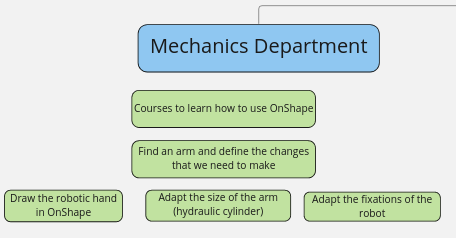
\includegraphics[width=0.8\textwidth]{Images/Section02/wbs.png}
    \caption{WBS example}
    \label{fig:WBSextract}
\end{figure}
\FloatBarrier

\bigbreak
Thanks to this document, we set up a \gls{gantt}\footnote{Graphical representation of a schedule} (appendix \ref{Gantt}). It illustrates the project schedule by indicating the tasks to be accomplished and the time. Each pole had its Gantt chart, which was linked to a global chart. This allowed us to anticipate certain delays and adapt. \Gls{milestone}\textcolor{SteelBlue}{s}\footnote{Siginificant stage or event in the development of something} were also defined in order to have objectives all along the project. Their dates were set on the audits during the project.

\begin{figure}[ht]
    \centering
    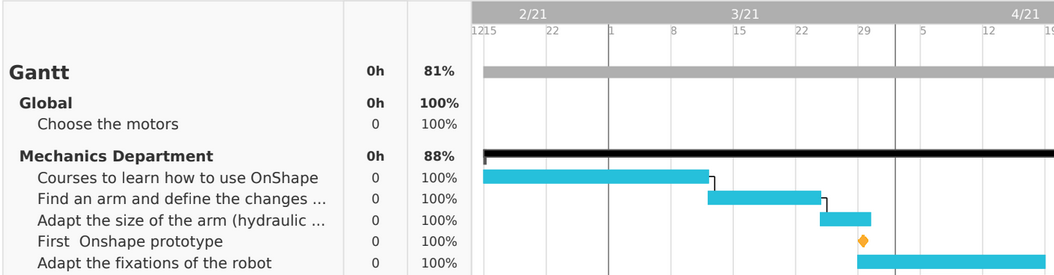
\includegraphics[width=0.8\textwidth]{Images/Section02/gantt.png}
    \caption{Gantt example}
    \label{fig:GANTTextract}
\end{figure}
\FloatBarrier

\bigbreak
Finally, to manage the daily tasks and ensure both a good distribution of work between members and their achievement we used a to-do-list. It indicated the tasks to be carried out, the person in charge, the person in charge who followed the progress, the date, and the status. 

\begin{figure}[ht]
    \centering
    \includegraphics[width=0.8\textwidth]{Images/Section02/to\_do\_list.png}
    \caption{To do list example}
    \label{fig:ToDoList}
\end{figure}

\subsection{Communication}

Communication was a key point for success. We were fortunate to have a client who was very involved in the project. Thus, we had weekly meetings with him to review the progress. It was also an opportunity to take advantage of his expertise in the management of such a project as well as his ideas. During those meetings, we discussed both the technical and management aspects. He also allowed us to meet people such as the CTO of BMW who gave us precious advice. At the request of Mr. Kedziora, we did not have a person in charge of taking notes. A schedule was defined in order to have a rotation between all the members and all benefit from this experience. A template for uniformity was set up. 

\bigbreak
Each pole also met one afternoon per week to work and exchange on the technical part of the project, and a monthly meeting was held between the pole managers and the project manager to ensure the smooth running of the project. 

\bigbreak
To exchange information, we had a Google Drive to store and share all the documents. GitHub folders were also created for the IT part. Finally, we also communicated with our client via Whatsapp. We also had a messenger group with all members. 

\subsection{Resource management}

Two types of means can be taken into account. First, the direct financial expenses. These are all the purchases we made. As explained earlier, Héloïse was responsible for this tracking. She could therefore easily ensure that the expenses were in line with the client's wishes. These expenses also included the use and purchase of materials from central offices. 

\begin{figure}[ht]
    \centering
    \includegraphics[width=0.8\textwidth]{Images/Section02/financial\_budget.png}
    \caption{Financial budget extract}
    \label{fig:financialBudgetextract}
\end{figure}
\FloatBarrier

\begin{figure}[ht]
    \centering
    \includegraphics[width=0.8\textwidth]{Images/Section02/material\_budget.png}
    \caption{Material budget extract}
    \label{fig:materialBudgetextract}
\end{figure}
\FloatBarrier
Many non-direct expenses were also taken into account. First, the cost of our work is summarized in the table below. But also the consulting hours. Indeed, Centrale offered the possibility to contact professors and benefit from their knowledge. So we contacted different people who redirected us to the teachers who could help us the most. To ensure full and balanced use as needed, Anna kept a document describing their use. 

\bigbreak
These hours were a great help. We were able to count on our coaches to help us manage this project. We were able to count on consultants, especially Mr. Kruszewski, who was really involved in the project. Thanks to him, we were able to benefit from an almost weekly follow-up to perpetually advance the project. It was also a question of privileged moments to deepen certain subjects with them.

\begin{figure}[ht]
    \centering
    \includegraphics[width=0.8\textwidth]{Images/Section02/human\_budget.png}
    \caption{Human budget extract}
    \label{fig:humanBudget}
\end{figure}